\themaN
\graphicspath{{../Ch4_Relations_d_ordre_sur_les_nombres/Images/}}

\chapter{Comparer\\des décimaux}
\label{C05}


%%%%%%%%%%%%%%%%%%%%%%%%%%%%%%%%%%%%%
\begin{prerequis}[Connaissances et compétences abordées]
   \begin{itemize}
      \item Repérer et placer un nombre décimal sur une demi-droite graduée adaptée.
      \item Comparer, ranger des nombres décimaux.
      \item Encadrer un nombre décimal par deux nombres entiers, par deux nombres décimaux.
      \item Trouver des nombres décimaux à intercaler entre deux nombres donnés.
      \item Connaître des procédures élémentaires de calcul, notamment : multiplier ou diviser un nombre décimal par 10, par 100, par 1000;
   \end{itemize}
\end{prerequis}

\vfill

\begin{debat}[Débat : vrai ou faux ?]
   \begin{enumerate}
      \item $4,26<4,249$ \hfill vrai \psframe(0,0)(0.25,0.25) \qquad faux \psframe(0,0)(0.25,0.25) \qquad \textcolor{white}{espace}
      \item $1,4 =1,40$ \hfill vrai \psframe(0,0)(0.25,0.25) \qquad faux \psframe(0,0)(0.25,0.25) \qquad \textcolor{white}{espace}
      \item 2,47 est le successeur de 2,46 \hfill vrai \psframe(0,0)(0.25,0.25) \qquad faux \psframe(0,0)(0.25,0.25) \qquad \textcolor{white}{espace}
      \item $2,3+7,12 =9,15$ \hfill vrai \psframe(0,0)(0.25,0.25) \qquad faux \psframe(0,0)(0.25,0.25) \qquad \textcolor{white}{espace}
      \item Entre 5 et 8, il y a une infinité de nombres décimaux \hfill vrai \psframe(0,0)(0.25,0.25) \qquad faux \psframe(0,0)(0.25,0.25) \qquad \textcolor{white}{espace}
   \end{enumerate}
   \bigskip
   \begin{center}
      \textcolor{B1}{\huge $1,11111>1,1111>1,111>1,11>1,1>1$}
   \end{center}
   \bigskip
   \begin{cadre}[B2][F4]
      \begin{center}
         Vidéo : \href{https://lesfondamentaux.reseau-canope.fr/discipline/mathematiques/nombres/comparer-les-decimaux/ranger-des-nombres.html}{\bf Ranger des nombres} du site {\it Canopé}, épisode de la série {\it Les fondamentaux}
      \end{center}
   \end{cadre}
\end{debat}

\vfill

\textcolor{PartieGeometrie}{\large\sffamily\bfseries Cahier de compétences} : chapitre 2, exercices 22 à 39.


%%%%%%%%%%%%%%%%%%%%%%%%%%%%%%%%%%%%
%%%%%%%%%%%%%%%%%%%%%%%%%%%%%%%%%%%%%
\activites

\begin{activite}[Avec une droite graduée, le retour !]
   {\bf Objectifs :} comparer, ordonner, encadrer, intercaler des nombres décimaux.
   \begin{QCM}
      \partie[réinvestissement]
         Reprendre la bande graduée du chapitre 3. \\
         Rappeler oralement la manière dont a été construire la graduation de la bande graduée. \\
         Quels sont les nombres qui ont été placés sur cette droite ? \\ [3mm]
         \pf \\ [5mm]
         \pf \\
         
      \partie[ordonner, encadrer, intercaler des nombres décimaux]
      
         \begin{enumerate}
            \item Écrire dans l'ordre croissant les nombres inscrits sur la droite graduée : \\ [3mm]
               \pf \\ [5mm]
               \pf \\
            \item Encadrer chacun des nombres suivants par deux nombres entiers consécutifs. \\
            \begin{colitemize}{3}
               \item \pfh < $\dfrac{8}{10}$ < \pfh \bigskip
               \item \pfh < 0,3 < \dashrulefill[0.5mm]{4 2}{0.15}  \bigskip
               \item \pfh < {\small cinq dixièmes} < \pfh \bigskip
               \item \pfh < $\dfrac{23}{10}$ < \pfh  \bigskip
               \item \pfh < 1,7 < \pfh
               \item \pfh < $2+\dfrac{1}{10}$ < \pfh
               \item \pfh < {\small douze dixièmes} < \pfh
               \item \pfh < $\dfrac{143}{100}$ < \pfh
               \item \pfh < $\dfrac{255}{100}$ < \pfh
               \item \pfh < 0,23 < \pfh
               \item \pfh < {\small 106 centièmes} < \pfh
               \item \pfh < $1+\dfrac{9}{10}+\dfrac{8}{100}$ < \pfh
            \end{colitemize}
            \item Encadrer chacun des nombres suivants par deux nombres décimaux séparés d'un dixième. \\
            \begin{colitemize}{3}
               \item \pfh < $\dfrac{143}{100}$ < \pfh \bigskip
               \item \pfh < $\dfrac{255}{100}$ < \pfh \bigskip
               \item \pfh < 0,23 < \pfh
               \item \pfh < {\small 106 centièmes} < \pfh
               \item \pfh < $1+\dfrac{9}{10}+\dfrac{8}{100}$ < \pfh
            \end{colitemize}
            \item \, Intercaler trois nombres entre : \medskip
            \begin{itemize}
               \item cinq dixièmes et $\dfrac{8}{10}$ : \pfb \\
               \item 2 et $2+\dfrac{1}{10}$ : \pfb \\
               \item 0,23 et 0,3 : \pfb
            \end{itemize}
         \end{enumerate}
   \end{QCM}
\end{activite}


%%%%%%%%%%%%%%%%%%%%%%%%%%%%%%%%%
%%%%%%%%%%%%%%%%% III %%%%%%%%%%%%%%%
\cours

\section{La droite graduée}

Si on partage l'unité d'une droite graduée en dix, on obtient des dixièmes; en partageant un dixième en dix, on obtient des centièmes \dots
      
\begin{center}   
   \begin{pspicture}(-2,-3)(11,1)
   {\psset{yunit=0.7}
      \small
      \rput(0,-1){
\includegraphics[width=3cm]{loupe}}
      \psaxes[yAxis=false]{->}(0,0)(10.3,0)
      \multido{\n=0.1+0.1}{9}{\psline[linewidth=0.01,linecolor=A1](\n,0.08)(\n,-0.08)}
      \psline[linestyle=dashed,linecolor=A1]{->}(0,0)(0,-2)
      \psline[linestyle=dashed,linecolor=A1]{->}(1,0)(10,-2)
      \psaxes[Dx=0.1,dx=1,comma,yAxis=false,linecolor=A1]{->}(0,-2)(10.3,-2)
      \multido{\n=0.1+0.1}{9}{\psline[linewidth=0.01,linecolor=B1](\n,-1.92)(\n,-2.08)}
      \psline[linestyle=dashed,linecolor=B1]{->}(0,-2)(0,-4)
      \psline[linestyle=dashed,linecolor=B1]{->}(1,-2)(10,-4)
      \psaxes[Dx=0.01,dx=1,comma,yAxis=false,linecolor=B1]{->}(0,-4)(10.3,-4)
      \multido{\n=0.1+0.1}{9}{\psline[linewidth=0.01](\n,-3.92)(\n,-4.08)}}
   \end{pspicture}
\end{center}


%%%%%%%%%%%%%%%%% III %%%%%%%%%%%%%%%
\section{Comparer des nombres décimaux}

\begin{methode}[Comparaison de deux nombres décimaux]
   Pour comparer deux nombres décimaux :
   \begin{itemize}
      \item je compare les parties entières ;
      \item si les parties entières sont égales, alors je compare les chiffres des dixièmes ;
      \item si les chiffres des dixièmes sont égaux, alors je compare les chiffres des centièmes et ainsi de suite jusqu’à ce que les deux nombres aient des chiffres différents.
   \end{itemize}
   \exercice
      Comparer 4,735 et 4, 74.  
   \correction
      Ils ont même partie entière, même chiffre des dixièmes mais un chiffre des centièmes différent : $3<4$ don $4,735<4,74$.
\end{methode}


%%%%%%%%%%%%%%%%%%%%%%%%%%%%%%%%%
\section{Ranger, encadrer, intercaler}

Tout comme les nombres entiers, on peut ranger, encadrer, intercaler des nombres décimaux.

\begin{exemple*1}
   \begin{itemize}
      \item $8,37<8,6<8,7$ sont rangés dans l'ordre croissant.
      \item $8,7>8,6>8,37$ sont rangés dans l'ordre décroissant.
      \item On peut encadrer $8,37$ par deux entiers consécutifs : $8<8,37<9$.
      \item On peut intercaler un nombre entre 8,6 et 8,7 : par exemple 8,63. \\
        \begin{pspicture}(0,-0.3)(11,0.7)
           {\psset{xunit=1.3}
           \small
           \rput(10,-0.45){9}
           \rput(10,0){|}
           \psaxes[yAxis=false,Ox=8,Dx=0.1,dx=1,comma,subticks=10]{->}(0,0)(10.15,0)
           \psline[linewidth=0.05,linecolor=violet,linestyle=dashed]{->}(0,0.5)(0,0)
           \psline[linewidth=0.05,linecolor=violet]{->}(3.7,0.5)(3.7,0) 
           \psline[linewidth=0.05,linecolor=violet,linestyle=dashed]{->}(10,0.5)(10,0)
           \psline[linewidth=0.05,linecolor=teal]{->}(7,0.5)(7,0)
           \psline[linewidth=0.05,linecolor=teal,linestyle=dashed]{->}(6.3,0.5)(6.3,0)
           \psline[linewidth=0.05,linecolor=teal]{->}(6,0.5)(6,0)}
        \end{pspicture}
   \end{itemize}
\end{exemple*1}

\begin{remarque}
   on peut intercaler autant de nombres que l'on veut entre deux nombres décimaux (on dit qu'il y en a une infinité). \\
   Par exemple, entre 8,6 et 8,7 on a 8,63, mais aussi 8,64 ; 8,699 ; 8, 675344355\dots
\end{remarque}


%%%%%%%%%%%%%%%%%%%%%%%%%%%%%%%%%%%%%%%%%%
\exercicesbase

\begin{colonne*exercice}

\serie{La droite graduée} %%%%%%%%%%%%%%%%%%%%

\begin{exercice} %1
   Écrire l'abscisse de chaque point.
   \begin{enumerate}
      \small
      \item \begin{pspicture}(0,0)(8,0.7)
                  \psset{xunit=5}
                  \psaxes[yAxis=false,subticks=10,subtickcolor=black]{->}(0,0)(1.5,0)
                  \pstGeonode[PosAngle=90](0.3,0){A}(0.8,0){B}(1.1,0){C}(1.3,0){D}
               \end{pspicture}
      \item \begin{pspicture}(0,0)(8,1.2)
                  \psset{xunit=5}
                  \psaxes[yAxis=false,Ox=12,subticks=10,subtickcolor=black]{->}(0.2,0)(1.5,0)
                  \psline(0,0)(0.2,0)
                  \psline[linewidth=0.07mm](0.1,0.1)(0.1,-0.1)
                  \pstGeonode[PosAngle=90](0.3,0){E}(0.5,0){F}(0.7,0){G}(1.3,0){H}
               \end{pspicture}
      \item \begin{pspicture}(0,0)(8,1.2)
                  \psset{xunit=1.1}
                  \psaxes[yAxis=false,Ox=24,subticks=2,subtickcolor=black,labels=none]{->}(0,0)(6.5,0)
                  \rput(1,-0.3){25}
                  \rput(2,-0.3){26}
                  \psline(0,0)(0.2,0)
                  \psline[linewidth=0.07mm](0.1,0.1)(0.1,-0.1)
                  \pstGeonode[PosAngle=90](1.5,0){J}(3.5,0){K}(5.5,0){L}
               \end{pspicture}
      \item \begin{pspicture}(0,0)(8,1.2)
                  \psset{xunit=0.45}
                  \psline{->}(0,0)(16,0)
                  \multido{\n=1+1}{15}{\psline[linecolor=darkgray,linewidth=0.1mm](\n,-0.1)(\n,0.1)}
                  \psline(2,-0.1)(2,0.1)
                  \rput(2,-0.35){7,8}
                  \psline(12,-0.1)(12,0.1)
                  \rput(12,-0.35){7,9}
                  \pstGeonode[PosAngle=90](3,0){M}(5,0){N}(11,0){P}(13,0){Q}
               \end{pspicture}
       \item \begin{pspicture}(0,0)(8,1.2)
                  \psset{xunit=0.45}
                  \psline{->}(0,0)(16,0)
                  \multido{\n=1+1}{15}{\psline[linecolor=darkgray,linewidth=0.1mm](\n,-0.1)(\n,0.1)}
                  \psline(4,-0.1)(4,0.1)
                  \rput(4,-0.35){6,41}
                  \psline(14,-0.1)(14,0.1)
                  \rput(14,-0.35){6,42}
                  \pstGeonode[PosAngle=90](2,0){V}(7,0){W}(10,0){Y}(12,0){Z}
               \end{pspicture}
   \end{enumerate}
\end{exercice}

%\begin{corrige}
%   \ \\ [-5mm]
%   \begin{enumerate}
%      \item $A({\blue 0,3}) \; ; \; B({\blue 0,8}) \; ; \; C({\blue 1,1}) \; ; \; D({\blue 1,3})$.
%      \item $E({\blue 12,1}) \; ; \; F({\blue 12,3}) \; ; \; G({\blue 12,5}) \; ; \; H({\blue 13,1})$.
%      \item $J({\blue 25,5}) \; ; \; K({\blue 27,5}) \; ; \; L({\blue 29,5})$.
%      \item $M({\blue 7,81}) \; ; \; N({\blue 7,83}) \; ; \; P({\blue 7,89}) \; ; \; Q({\blue 7,91})$.
%      \item $V({\blue 6,408}) \; ; \; W({\blue 6,413}) \; ; \; Y({\blue 6,416}) \; ; \; Z({\blue 6,418})$.
%   \end{enumerate}
%\end{corrige}

\bigskip

\begin{exercice}
   Placer les points donnés sur chaque droite.
   {\psset{unit=0.9}
   \small
   \begin{enumerate}
      \item A(11,5) \; ; \; B(8,5) \; ; \; C(9,7) \; et \; D(8,1). \\
        \begin{pspicture}(0.3,-0.5)(8,1.2)
           \milli{0}{-0.5}{8}{1}
           \psaxes[yAxis=false,Dx=2,labels=none]{->}(0,0)(8,0)
           \rput(2,-0.35){9}
           \rput(4,-0.35){10}
        \end{pspicture}
      \item E(0,2) \; ; \; F(0,55) \; ; \; G(0,73) \; et \; H(0,40). \\
        \begin{pspicture}(0.3,-0.5)(8,1.2)
           \milli{0}{-0.5}{8}{1}
           \psaxes[yAxis=false,labels=none]{->}(0,0)(8,0)
           \rput(2,-0.35){0,3}
           \rput(3,-0.35){0,4}
        \end{pspicture}
     \item J(5,33) \; ; \; K(5,28) \; ; \; L(5,315) \; et \; M(5,304). \\
        \begin{pspicture}(0.3,-0.5)(8,1.2)
           \milli{0}{-0.5}{8}{1}
           \psaxes[yAxis=false,Dx=1,labels=none]{->}(0,0)(8,0)
           \rput(3,-0.35){5,3}
           \rput(4,-0.35){5,31}
        \end{pspicture}
   \end{enumerate}}
\end{exercice}


\serie{Comparer des nombre décimaux} %%%%%%%%%%%%%


\medskip

\begin{exercice} %3
   Compléter avec le signe < ou >. \medskip
   \begin{colenumerate}{2}
      \item 15,1 \pfh 15,09 \smallskip
      \item 132,45 \pfh 132,46 \smallskip
      \item 7,101 \pfh 17,011 \smallskip
      \item 435,6 \pfh 438,6
      \item 5,126 \pfh 5,1236
      \item 6,048 \pfh 6,15
   \end{colenumerate}
\end{exercice}

%\begin{corrige}
%   \begin{colenumerate}{2}
%      \item 15,1 {\blue\,>\,} 15,09 \smallskip
%      \item 132,45 {\blue\,<\,} 132,46 \smallskip
%      \item 7,101 {\blue\,>\,} 17,011 \smallskip
%      \item 435,6 {\blue\,<\,} 438,6 \smallskip
%      \item 5,126 {\blue\,>\,} 5,1236
%      \item 6,048 {\blue\,<\,} 6,15
%      \item 8,75 {\blue\,<\,} 8,9
%      \item 19,47 {\blue\,>\,} 19,435
%   \end{colenumerate}
%\end{corrige}

\begin{exercice} %2
   Compléter avec le signe < ou >. \medskip
   \begin{colenumerate}{2}
      \item $\dfrac{32}{100} \pfh \dfrac{40}{100}$ \medskip
      \item $\dfrac{7}{10} \pfh \dfrac{7}{100}$ \medskip
      \item $\dfrac{43}{100} \pfh \dfrac{4}{10}$ \medskip
      \item $\dfrac{37}{100} \pfh \dfrac{307}{1\,000}$
      \item $5+\dfrac{8}{10} \pfh 5+\dfrac{8}{100}$
      \item $3+\dfrac{2}{10} \pfh 3+\dfrac{22}{100}$
   \end{colenumerate}
\end{exercice}

%\begin{corrige}
%   \begin{colenumerate}{2}
%      \item $\dfrac{32}{100} {\blue\,<\,} \dfrac{40}{100}$ \medskip
%      \item $\dfrac{7}{10} {\blue\,>\,} \dfrac{7}{100}$ \medskip
%      \item $\dfrac{43}{100} {\blue\,>\,} \dfrac{4}{10}$ \medskip
%      \item $\dfrac{85}{100} {\blue\,<\,} \dfrac{9}{10}$
%      \item $\dfrac{37}{100} {\blue\,>\,} \dfrac{307}{1\,000}$
%      \item $5+\dfrac{8}{10} {\blue\,>\,} 5+\dfrac{8}{100}$
%      \item $3+\dfrac{2}{10} {\blue\,<\,} 3+\dfrac{22}{100}$
%      \item $\dfrac{7\,859}{1\,000} {\blue\,<\,} 78+\dfrac{59}{100}$
%   \end{colenumerate}
%\end{corrige}


\serie{Ranger, encadrer, intercaler} %%%%%%%%%%%%%%%%%%

\begin{exercice}
   Ranger chaque série de nombres :
   \begin{enumerate}
      \item dans l'ordre croissant. \smallskip
      \begin{enumerate}
         \item \fbox{4,99} \; \fbox{4,9} \; \fbox{4,88} \; \fbox{5,01} \; \fbox{4,909} \; \fbox{4,879} \smallskip
         \item \fbox{0,7} \; \fbox{0,07} \; \fbox{0,707} \; \fbox{0,007} \; \fbox{0,77} \; \fbox{0,077}
      \end{enumerate}
      \item dans l'ordre décroissant. \smallskip
      \begin{enumerate}
         \item \fbox{1,28} \; \fbox{1,82} \; \fbox{1,028} \; \fbox{1,8} \; \fbox{1,282} \; \fbox{1,2} \smallskip
         \item \fbox{5,3} \; \fbox{3,5} \; \fbox{5,35} \; \fbox{3,53} \; \fbox{5,353} \; \fbox{3,535}
      \end{enumerate}
   \end{enumerate}
\end{exercice}

%\begin{corrige}
%   \ \\ [-5mm]
%   \begin{enumerate}
%      \item \blue 0,007 \, < \, 0,07 \, < \, 0,077 \, < \, 0,7 \, < \, 0,707 \, < \, 0,77
%      \item 5,353 \, > \, 5,35 \, > \, 5,3 \, > \, 3,535 \, > \, 3,53 \, > \, 3,5
%   \end{enumerate}
%\end{corrige}

\begin{exercice} %17
   Classer dans l'ordre croissant l'ensemble de ces lettres afin de trouver le mot mystère.
   \begin{colitemize}{3}
      \item I = 65,165
      \item S = $\dfrac{655}{10}$
      \item B = $\dfrac{6\,503}{100}$
   \end{colitemize}
   \begin{colitemize}{2}
      \item A = $56+\dfrac{6}{100}$
      \item M = $50+6+\dfrac{65}{1\,000}$
      \item O = $\dfrac{651}{10}+\dfrac{3}{100}$
      \item R = $56+\dfrac{5}{100}$
   \end{colitemize}
   \begin{colitemize}{1}
      \item E = $(6\times10)+(5\times1)+(6\times0,1)$
      \item F = 56 unités et 6 millièmes
   \end{colitemize}
\end{exercice}
%
%\begin{corrige}
%   \begin{colitemize}{3}
%      \item I = 65,165
%      \item S = 65,5
%      \item B = 65,03
%      \item A = 56,06
%      \item O = 65,13
%      \item M = 56,065
%      \item R = 56,05
%      \item E = 65,6
%      \item F = 56,006
%   \end{colitemize}
%   On a $65,006 < 56,05 < 56,06 < 56,065 < 65,03 < 65,13 < 65,165 < 65,5 < 65,6$. \\
%   Conclusion : le mot mystère est \blue FRAMBOISE.
%\end{corrige}

\medskip

\begin{exercice} %5
   Encadrer ces nombres par deux nombres décimaux séparés d'un dixième.
   \begin{colenumerate}{2}
      \item \pfh < 8,51 < \pfh
      \item \pfh < 99,01 < \pfh
      \item \pfh < 0,956 < \pfh
      \item \pfh < 29,108 < \pfh
      \item \pfh < 123,19 < \pfh
      \item \pfh < 77,777 < \pfh
   \end{colenumerate}
\end{exercice}

%\begin{corrige}
%   \begin{colenumerate}{2}
%      \item {\blue 8,5} < 8,51 < {\blue 8,6}
%      \item {\blue 99} < 99,01 < {\blue 99,1}
%      \item {\blue 0,9} < 0,956 < {\blue 1}
%      \item {\blue 29,1} < 29,108 < {\blue 29,2}
%      \item {\blue 123,1} < 123,19 < {\blue 123,2}
%      \item {\blue 77,7} < 77,777 < {\blue 77,8}
%   \end{colenumerate}
%\end{corrige}

\medskip


\begin{exercice} %10
   Intercaler un nombre décimal entre les deux nombres donnés.
   \begin{colenumerate}{2}
      \item 57 < \pfh < 58
      \item 0,6 < \pfh < 0,61
      \item 8,4 < \pfh < 8,5
      \item 5,12 < \pfh < 5,123
      \item 74,1 < \pfh < 74,2
      \item 45,78 < \pfh < 45,781
   \end{colenumerate}
\end{exercice}

%\begin{corrige}
%   On a, par exemple (solutions non uniques) :
%   \begin{colenumerate}{2}
%      \item 57 < {\blue 57,5} < 58
%      \item 0,6 < {\blue 0,607} < 0,61
%      \item 8,4 < {\blue 8,41} < 8,5
%      \item 5,12 < {\blue 5,122} < 5,123
%      \item 74,1 < {\blue 74,13} < 74,2
%      \item {\small 45,78 < {\blue 45,7806} < 45,781}
%   \end{colenumerate}
%\end{corrige}

\medskip


\begin{exercice} %12
   Quel pingouin vérifie les caractéristiques suivantes (justifier) :
   \begin{itemize}
      \item il mesure entre \um{0,75} et \um{0,85} ;
      \item il pèse entre \ukg{4,8} et \ukg{5,2} ;
      \item il a moins de 10 ans.
   \end{itemize}
  \begin{center}
      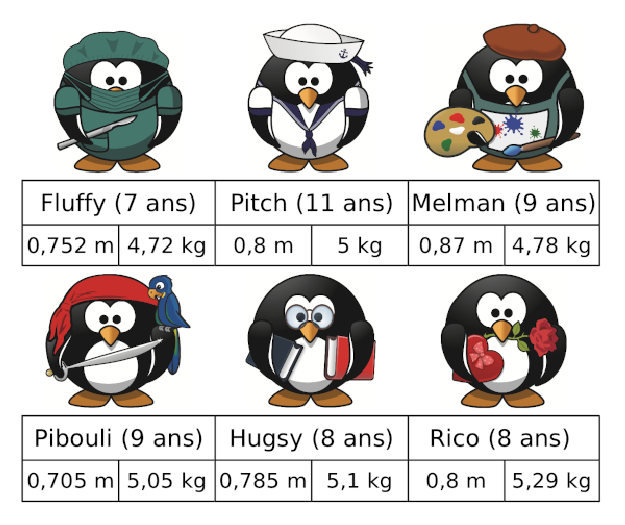
\includegraphics[width=5.5cm]{pingouin}
   \end{center}
\end{exercice}

%\begin{corrige}
%   \begin{itemize}
%      \item Le pingouin doit mesurer entre \um{0,75} et \um{0,85} donc, on peut éliminer Melman et Pibouli.
%      \item Le pingouin doit peser entre \ukg{4,8} et \ukg{5,2} donc, on peut éliminer Fluffy, Melman et Rico.
%      \item Le pingouin doit avoir moins de 10 ans donc, on peut éliminer Pitch.
%   \end{itemize}
%   Conclusion : {\blue on choisit Hugsy}. \\
%\end{corrige}

\end{colonne*exercice}


%%%%%%%%%%%%%%%%%%%%%%%%%%%%%%%%%%%%%%%
%%%%%%%%%%%%%%%%%%%%%%%%%%%%%%%%%%%%%%%
\Recreation

\enigme[Nombres croisés]
   \partie[mode d'emploi]
      Une grille de nombres croisés se comporte comme une grille de mots croisés :
      \begin{itemize}
         \item horizontalement, les lignes sont repérées par des chiffres romains de I à V ;
         \item verticalement, les colonnes sont repérées par des lettres de A à E ;
         \item les indications des nombres à trouver sont indiquées sous la grille de nombres croisés, repérées par des chiffres romains ou des lettres selon s'ils sont horizontaux ou verticaux ;
         \item il est interdit d'écrire dans les cases noires ;
         \item lorsqu'une ligne ou une colonne ne possède pas de carré noir, il y a un seul nombre à écrire ;
         \item lorsqu'une ligne ou une colonne possède un carré noir, il y a deux nombres à écrire, ces deux nombres sont définis par deux lignes différentes. \\
      \end{itemize}
      
   \partie[let's go !]
Compléter la grille à l'aide de nombres entiers correspondant aux définitions.
   \begin{center}
      {\psset{unit=1.2}\begin{pspicture}(-1,-0.5)(5,5.8)
         \psgrid[gridlabels=0,subgriddiv=0](0,0)(5,5)
         \psframe[fillstyle=solid,fillcolor=black](0,0)(1,1)
         \psframe[fillstyle=solid,fillcolor=black](4,1)(5,2)
         \psframe[fillstyle=solid,fillcolor=black](1,2)(2,3)
         \psframe[fillstyle=solid,fillcolor=black](3,4)(4,5)
         \rput(0.5,5.4){\bf A}
         \rput(1.5,5.4){\bf B}
         \rput(2.5,5.4){\bf C}
         \rput(3.5,5.4){\bf D}
         \rput(4.5,5.4){\bf E}
         \rput(-0.4,0.5){\bf V}
         \rput(-0.4,1.5){\bf IV}
         \rput(-0.4,2.5){\bf III}
         \rput(-0.4,3.5){\bf II}
         \rput(-0.4,4.5){\bf I}
      \end{pspicture}}
   \end{center}
   \begin{multicols}{2}
      {\bf Horizontalement} \\ [3mm]
         {\bf I} : Partie entière de 328,54. \\
         \hspace*{2.7mm} Chiffre des centièmes de 634,152. \\ [2mm]
         {\bf II} : Son chiffre des dizaines est le triple \\
         \hspace*{4mm} de celui des unités. \\ [2mm]
         {\bf III} : Chiffre des dixièmes de 34. \\
         \hspace*{5.6mm} Entier précédant 178,356. \\ [2mm]
         {\bf IV} : Entier compris entre 8\,000 et 9\,000. \\ [2mm]
         {\bf V} : Quarante-deux centaines. \\ [5mm]
      {\bf Verticalement} \\ [3mm]
        {\bf A} : $(3\times1 000) + (5\times100) + (8\times1)$. \\ [2mm]
        {\bf B} : Nombre de dixièmes dans 2,6. \\ [1mm]
        \hspace*{4mm} Partie entière de $\dfrac{2\,498}{100}$. \\ [3mm]
        {\bf C} : Quatre-vingt-six milliers et cent-deux unités. \\ [2mm]
        {\bf D} : En additionnant tous les chiffres \\
        \hspace*{4.5mm} du nombre, on trouve 20. \\ [2mm]
        {\bf E} : Entier qui suit 537,56. \\
        \hspace*{3.5mm} Entier qui précède 1. \\
     \end{multicols}
